\chapter{Ergebnisse}


\section{Relacsauswertung}


\begin{figure}[ht]
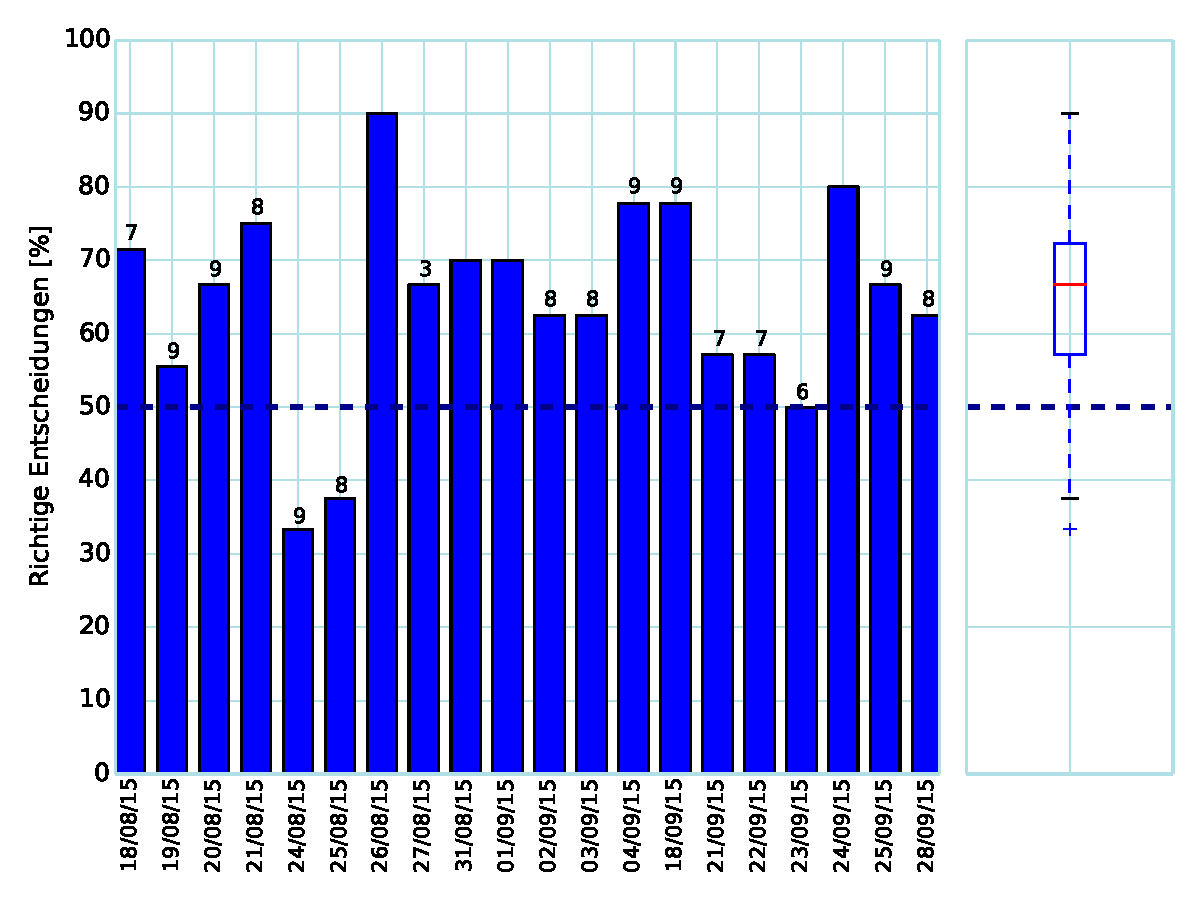
\includegraphics[height=6.5cm]{Abbildungen/Amplitude1_Fisch1}
\caption{\label{fig:amplitude1_1} Performance bei Amplitude 1 Fisch 1 mit Boxplot der mittleren Performance}
\end{figure}

\begin{figure}[ht]
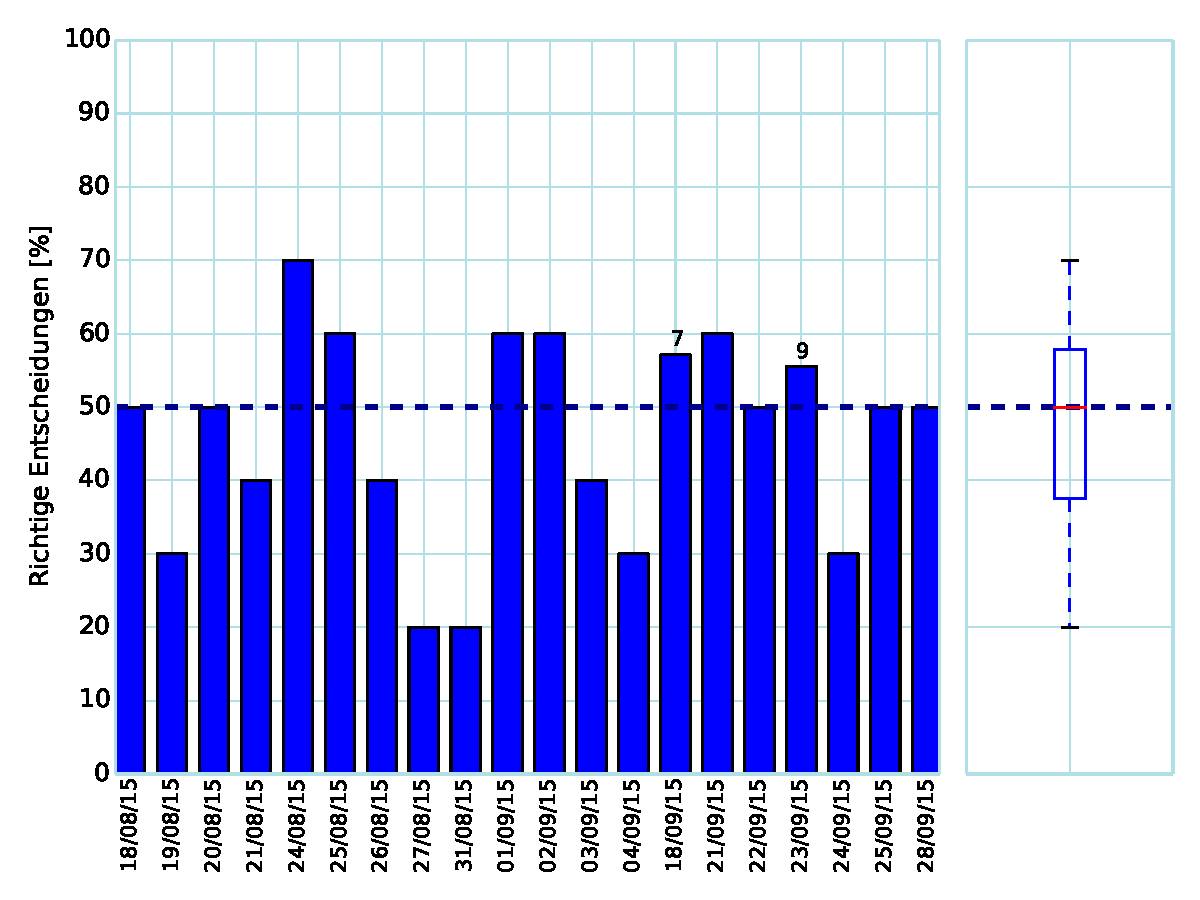
\includegraphics[height=6.5cm]{Abbildungen/Amplitude1_Fisch2}
\caption{\label{fig:amplitude1_2} Performance bei Amplitude 1 Fisch 2 mit Boxplot der mittleren Performance}
\end{figure}

\begin{figure}[ht]
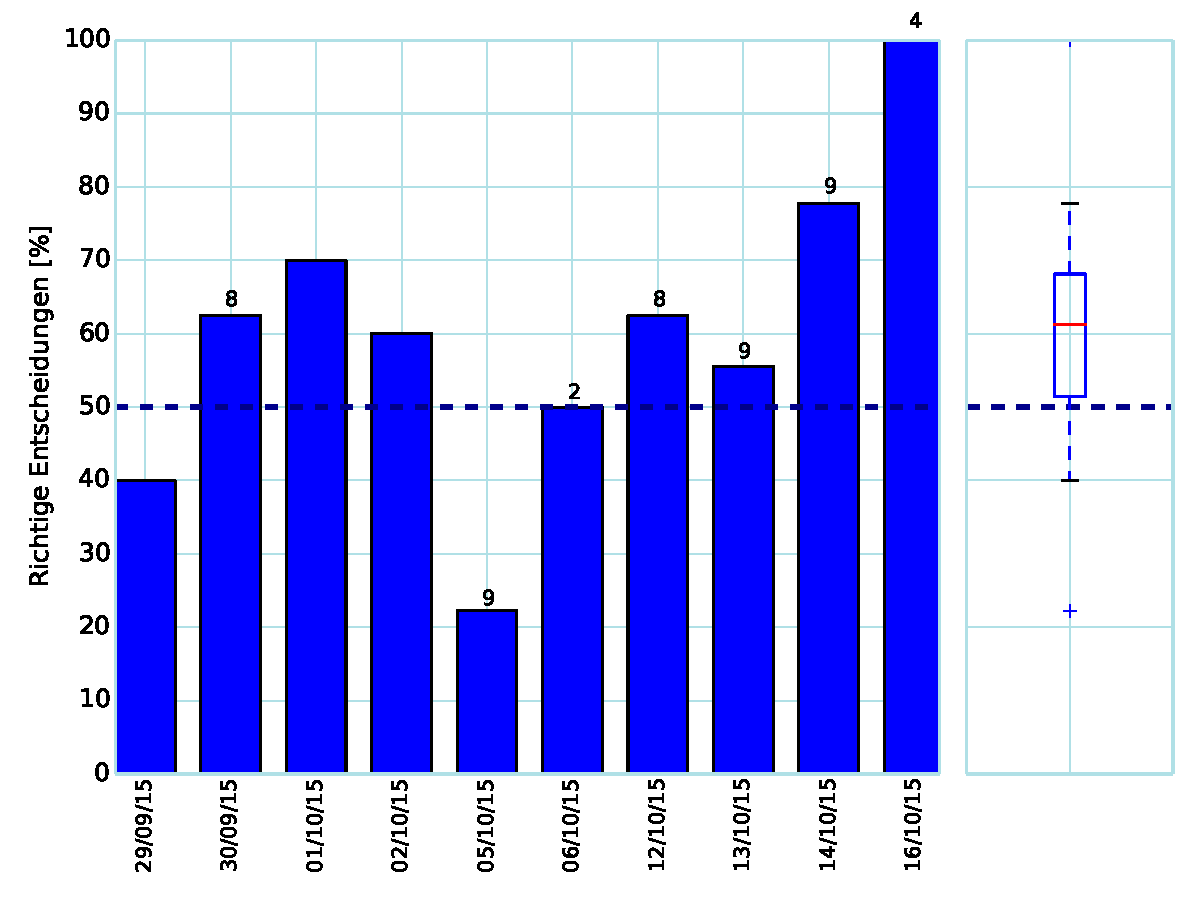
\includegraphics[height=6.5cm]{Abbildungen/Amplitude2_Fisch1}
\caption{\label{fig:amplitude2_1} Performance bei Amplitude 2 Fisch 1 mit Boxplot der mittleren Performance}
\end{figure}

\begin{figure}[ht]
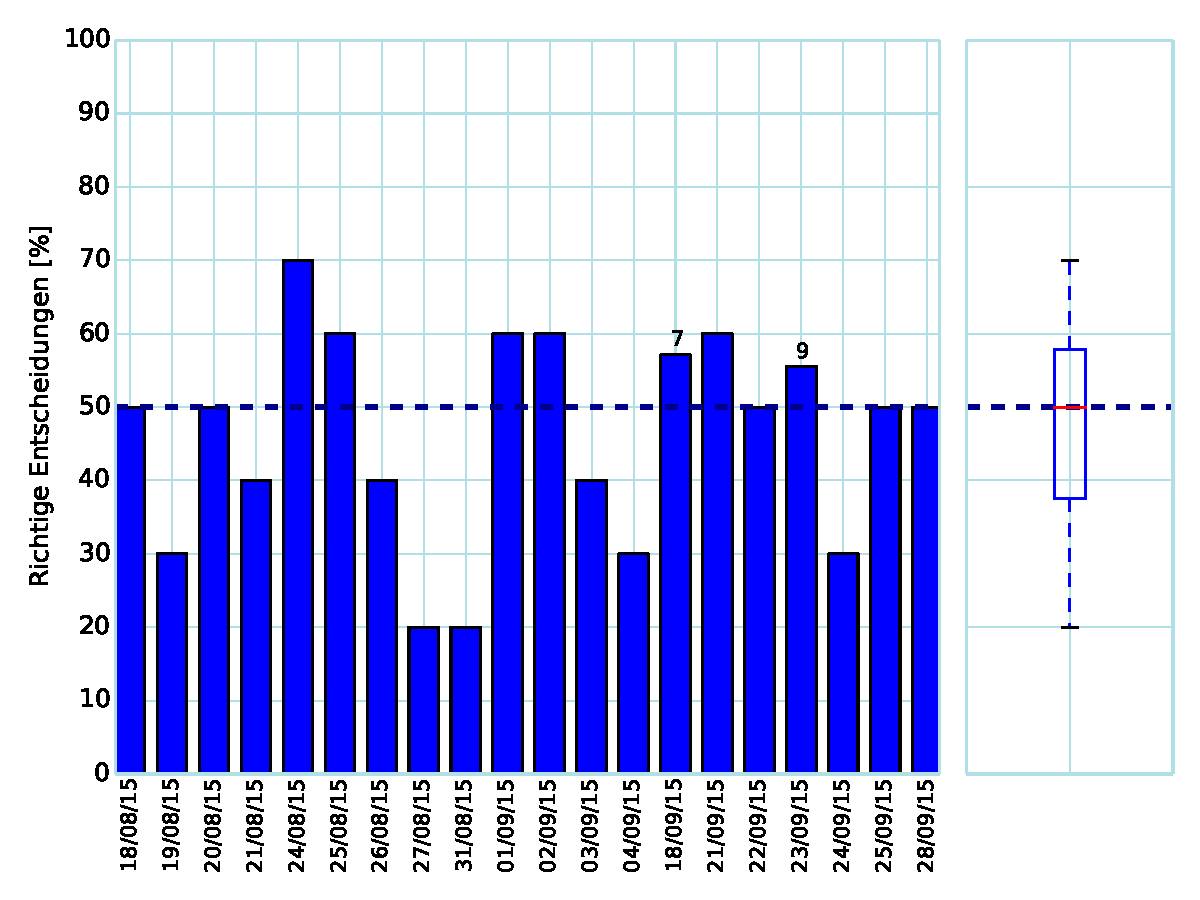
\includegraphics[height=6.5cm]{Abbildungen/Amplitude1_Fisch2}
\caption{\label{fig:amplitude2_2} Performance bei Amplitude 2 Fisch 2 mit Boxplot der mittleren Performance}
\end{figure}

\begin{figure}[ht]
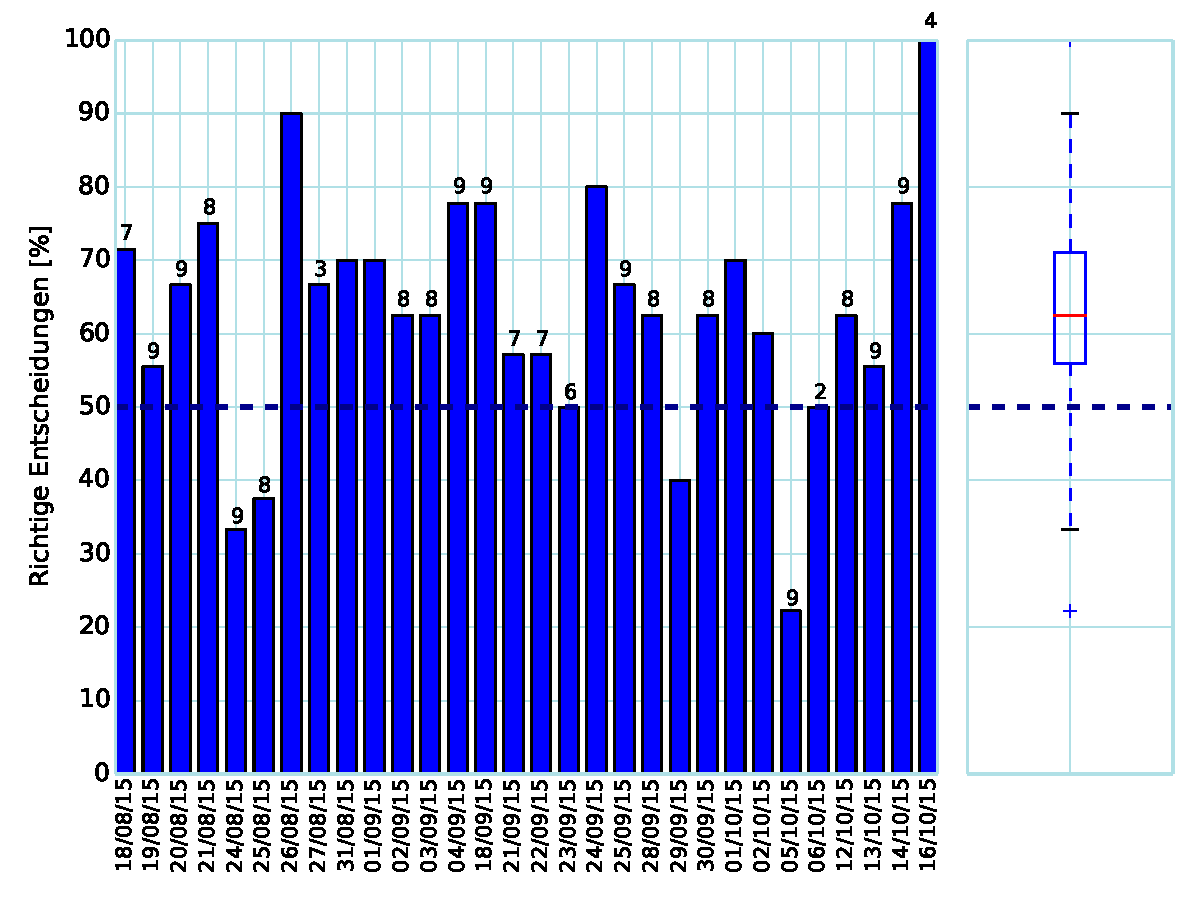
\includegraphics[height=6.5cm]{Abbildungen/Overview1}
\caption{\label{fig:amplitude1_1}Overview Fisch 1 mit Boxplot}
\end{figure}

\begin{figure}[ht]
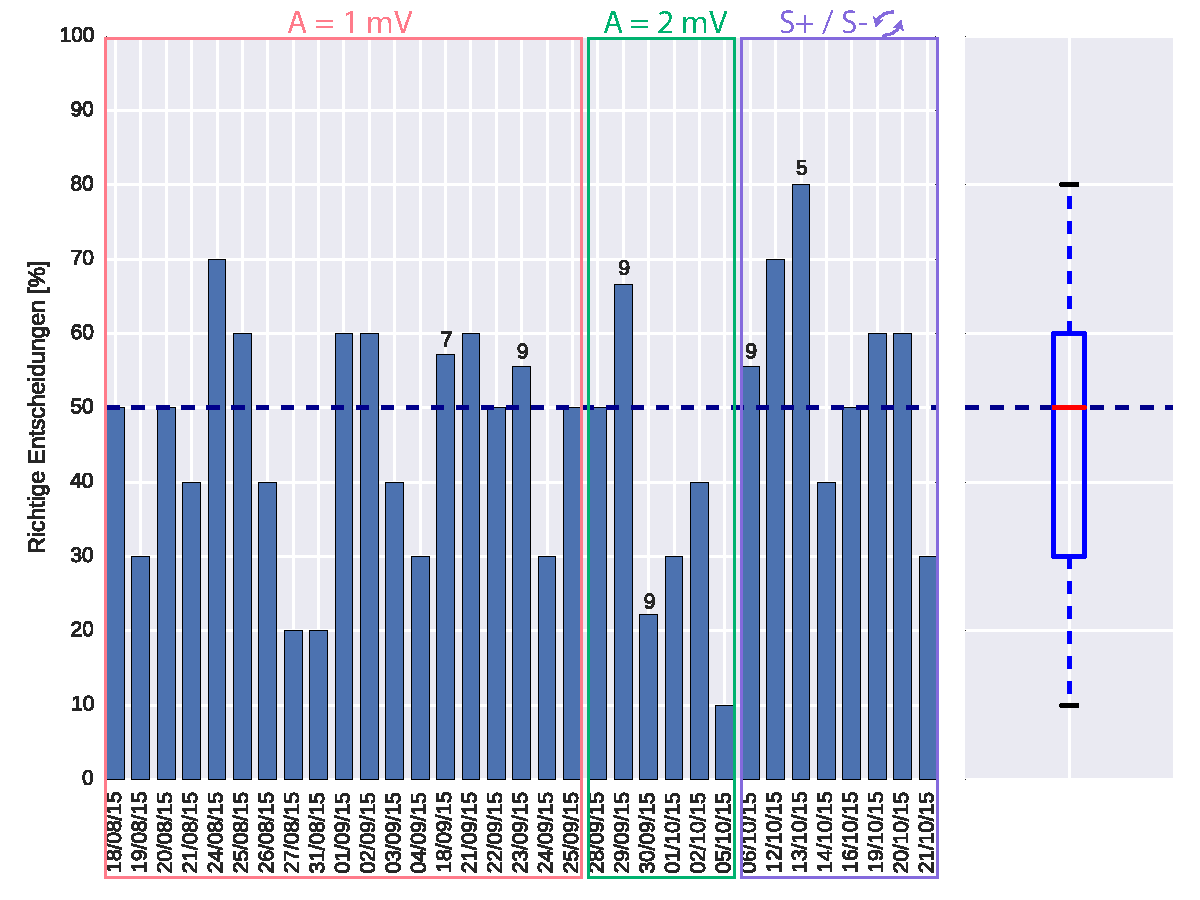
\includegraphics[height=6.5cm]{Abbildungen/Overview2}
\caption{\label{fig:amplitude1_1}Overview Fisch 2 mit Boxplot}
\end{figure}

\begin{figure}[ht]
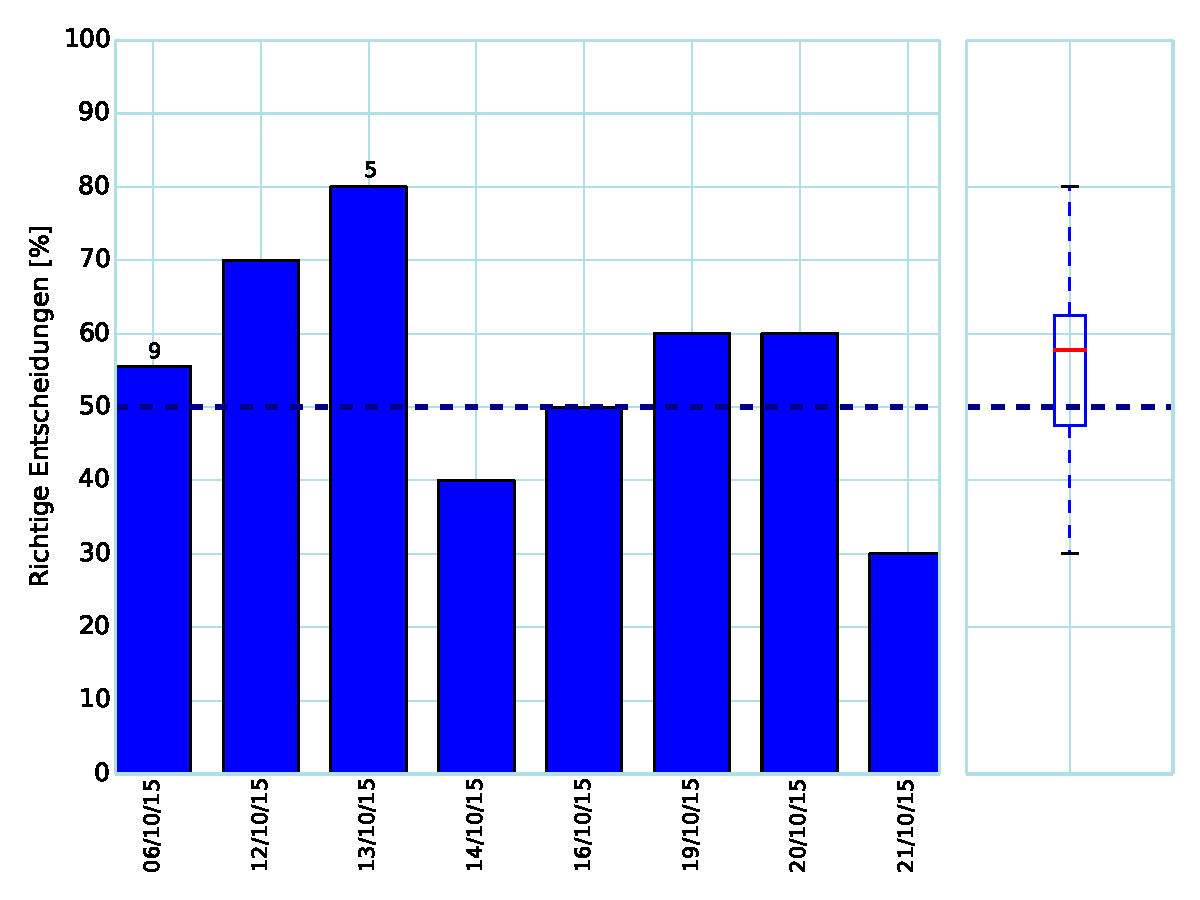
\includegraphics[height=6.5cm]{Abbildungen/getauschte_Stimuli}
\caption{\label{fig:amplitude1_1}Overview Fisch 1 mit Boxplot}
\end{figure}





\section{Videotrackingauswertung}
\section{Auswertung der Vorversuche}